\documentclass[journal]{IAENGtran}

\ifCLASSINFOpdf
   \usepackage[pdftex]{graphicx}
  % declare the path(s) where your graphic files are
  % \graphicspath{{../pdf/}{../jpeg/}}
  % and their extensions so you won't have to specify these with
  % every instance of \includegraphics
   \DeclareGraphicsExtensions{.pdf,.jpeg,.png}
\else
  % or other class option (dvipsone, dvipdf, if not using dvips). graphicx
  % will default to the driver specified in the system graphics.cfg if no
  % driver is specified.
   \usepackage[dvips]{graphicx}
  % declare the path(s) where your graphic files are
  % \graphicspath{{../eps/}}
  % and their extensions so you won't have to specify these with
  % every instance of \includegraphics
   \DeclareGraphicsExtensions{.eps}
\fi

\begin{document}
%
% paper title
% can use linebreaks \\ within to get better formatting as desired
% ユーザの既訪問スポットの位置づけに基づく未訪問スポットの説明手法
\title{An Explanation Method of Unfamiliar Tourist Spots based on Roles of User's Familiar Spots}
%
%
% author names and IAENG memberships
% note positions of commas and nonbreaking spaces ( ~ ) LaTeX will not break
% a structure at a ~ so this keeps an author's name from being broken across
% two lines.
% use \thanks{} to gain access to the first footnote area
% a separate \thanks must be used for each paragraph as LaTeX2e's \thanks
% was not built to handle multiple paragraphs
%

\author{Kenta~Han and Daisuke~Kitayama

% \thanks{Manuscript received January 8, 2017; revised February 3, 2017. }
\thanks{K. T. Han is with the Graduate School of Engineering, Kogakuin University, Japan; e-mail: em18011@ns.kogakuin.ac.jp.}% <-this % stops a space
\thanks{D. Kitayama is with the Faculty of Informatics, Kogakuin University, Japan;  e-mail: kitayama@cc.kogakuin.ac.jp.}}% <-this % stops a space

\maketitle

\pagestyle{empty}
\thispagestyle{empty}

%%%%%%%%%%%%%%%%%%%%%%%%%%%%%%%%%%%%%%%%%%
%%%%%%%%%%%%%%%%%%%%%%%%%%%%%%%%%%%%%%%%%%
\begin{abstract}
% 近年,観光スポットを決める時にWeb上の観光情報を活用して計画を立てることが多くなっている.
In recent years, when user plans to travel, users often use tourist information on the Web.
% しかし,ユーザが多くのエリアから訪問したいエリアを決めた上で,さらに自分のイメージに合う観光スポットを探すのは膨大な時間と労力を必要とする.
However, travel often goes to an unfamiliar area, therefore it is difficult to get the tourist information properly.
% 本研究では,ユーザの未知なスポットに対する理解を支援するためには,既に訪問したことがある観光スポットの特徴を未訪問スポットにあてはめて理解を支援する説明手法を提案する.
Therefore, in order to support understanding of users' unfamiliar spots, we propose a method to explain tourist spots of unfamiliar area using tourist spots that have visited by users.
% 本研究では,まず,観光スポットのユーザレビューを用いて特徴ベクトルを生成する.
In this paper, at first, we generate the feature vector using user reviews of the tourist spot.
% 次に,既に訪問したスポットと比較した差分ベクトルを用いて,観光スポットの独特な特徴を抽出する.
Next, we use the relative feature vector compared with already visited spots to extract the role of the tourist spot for the user.
% 最後に,差分ベクトルの類似度に基づいて既訪問スポットと未訪問スポットの関連づけし,その関係を説明するためのキーワードを抽出する.
Finally, we associate the visited spot with the unfamiliar spot by the similarity of the relative feature vector, and further extract keywords that explain the relation.
% また,プロトタイプシステムを構築し,既訪問スポットと未訪問スポットとの説明情報の効果を検証する評価実験を行う.
We also develop the prototype system, and we evaluate the effect of the explanatory information between the familiar spot and the unfamiliar spot.
\end{abstract}

%%%%%%%%%%%%%%%%%%%%%%%%%%%%%%%%%%%%%%%%%%
%%%%%%%%%%%%%%%%%%%%%%%%%%%%%%%%%%%%%%%%%%
\begin{IAENGkeywords}
% 観光スポット,理解支援,レビュー,分散表現
tourist spots, explainability, user reviews, paragraph vector
\end{IAENGkeywords}

\IAENGpeerreviewmaketitle


%%%%%%%%%%%%%%%%%%%%%%%%%%%%%%%%%%%%%%%%%%
%%%%%%%%%%%%%%%%%%%%%%%%%%%%%%%%%%%%%%%%%%
\section{Introduction}
\label{sec:Introduction}
%%%%%%%%%%%%%%%%%%%%%%%%%%%%%%%%%%%%%%%%%%
%%%%%%%%%%%%%%%%%%%%%%%%%%%%%%%%%%%%%%%%%%
% 旅行先を決定する時,旅行者は観光スポット検索サイトや観光情報に関連する書籍を見て観光スポットを選び,旅行計画を立てる.
\IAENGPARstart{W}{hen} deciding the travel destination, the traveler selects tourist spots by planning a travel, browsing web pages of tourist spots and tourist guidebooks.
% しかし,ユーザにとって訪問したいエリアを決定した後,さらにエリア内に数多く存在する観光スポットから,自身のイメージから外れない観光スポットを見つけることは容易ではない.
However, travel often goes to an unfamiliar area, therefore it is difficult to get the tourist information properly.
% このとき,行きたい観光スポットが決まっていない場合ではランキングやおすすめ情報を見て観光スポットを決めることが多くなると考えられる.
At this time, it is considered that the user often decides the tourist spot by looking at the ranking and recommendation information of the tourist spot search engine.
% Tripadvisorやじゃらんなどの観光スポット検索サイトでは,ユーザが特定の観光スポットを訪問した後レビューを投稿するため,観光スポットに関する報復な情報がある.
In a tourist spot search engine such as Tripadvisor and Jalan, the user who visited there about a certain tourist spot posted reviews and there is a wealth of information on tourist spots.
% しかし,ユーザは訪問したいエリアについての事前知識がないため,検索された観光スポットを1つずつ確認する必要がある.
However, since the user has no prior knowledge about the search area, what kind of tourist spot is to be confirmed one by one.
% さまざまな観光スポットを効果的に理解するためには,既存の情報をもとにして,未知な情報と既知な情報との対応関係を考えることが不可欠となる.
Therefore, in order to effectively understand various tourist spots, we think that it is effective if we compare an unfamiliar spot using a visited spot of user.
% この考え方は,以前に経験した事柄(ベースと呼ぶ)を,現在直面している事柄あるいは問題(ターゲットと呼ぶ)にあてはめる類推に相当する.
This is a kind of analogy that applies the matters that the user previously experienced to the current matter. In this case, the previous experience is the already visited spot and the current matter is the spot in the unfamiliar area.
% たとえば,金沢の「にし茶屋街」という未知なスポットに対して既訪問の京都の「花見小路」と似ていると説明するとイメージの理解がしやすくすることがある.
For example, whereas unfamiliar spots such as ``Omotesando'' in Tokyo, Japan, if you explain that it is similar to the already visited ``Avenue des Champs-Elysees'' in Paris, it may make it easier to understand.

% 本研究では,ユーザの未訪問スポットに対する理解を支援するため,既に訪問したことがある観光スポットの特徴を未訪問スポットにあてはめて理解を支援する説明手法を提案する.
In this paper, in order to support understanding of users' unfamiliar spots, we propose a method to explain tourist spots of unfamiliar area using tourist spots that have visited by users.
% 具体的には,ユーザが入力した既訪問スポットと未訪問エリアから,レビュを用いて既訪問スポット内の各スポットの独特な特徴と未訪問エリア内の各スポットの独特な特徴を抽出し,比較を行って説明情報を提示する.
% 具体的には,ユーザは既に訪問したスポットおよび未訪問エリアを入力する.
In our method, the user inputs already visited spots and unfamiliar area.
% そのとき,観光スポットのユーザレビューを用いて特徴ベクトルを生成する.
At this time, we generate the feature vector using user reviews of the tourist spot.
% 次に,既に訪問したスポットと比較した差分ベクトルを用いて,観光スポットの独特な特徴を抽出する.
Next, we use the relative feature vector compared with already visited spots to extract the role of the tourist spot for the user.
% 最後に,差分ベクトルの類似度に基づいて既訪問スポットと未訪問スポットの関連づけし,その関係を説明するためのキーワードを抽出する.
Finally, we associate the visited spot with the unfamiliar spot by the similarity of the relative feature vector, and further extract keywords that explain the relation.
By this way, we aim to rise understandability of unfamiliar spots.
% このプロトタイプシステムにより,ユーザが未訪問スポットに対する理解の支援を目指す.
%With this prototype system, users aim to support understanding of unfamiliar spots.
% 図\ref{fig:Photo_Image}は提案手法の概念図である.
Fig. \ref{fig:Photo_Image} shows a concept of the proposed method.

% 本論文の構成は下記のとおりである.2節では関連研究について述べる.3節では提案手法の概要について述べる.4節では構築したプロトタイプシステムの効果を検証する評価実験と考察について述べる.最後に5節ではまとめと今後の課題について述べる.
The structure of this paper is as follows.
In section \ref{sec:Related Work}, we introduce related works.
In section \ref{sec:An Explainaton Method of Unfamiliar Tourist Spots}, we describe the proposed method.
In section \ref{sec:Evaluation Experiment}, we discuss evaluation experiments and its results.
In section \ref{sec:Conclusions and Future Work}, we describe conclusions of this paper and our future work.

\begin{figure}[t]
  \begin{center}
    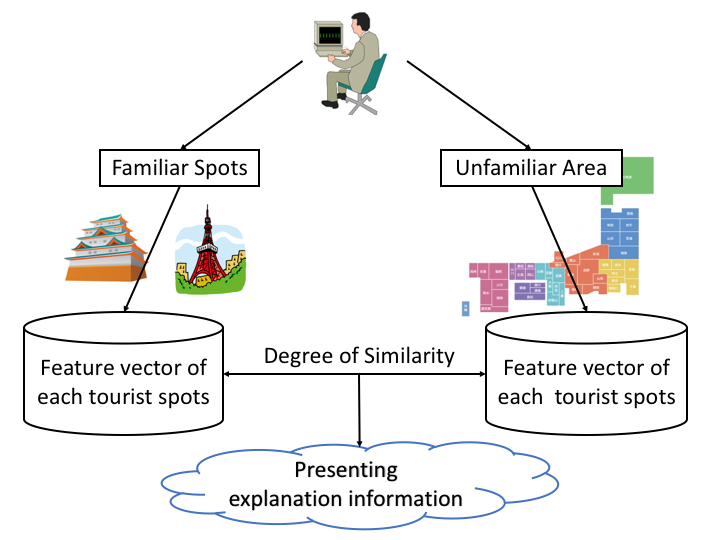
\includegraphics[clip,width=7.5cm,bb=0 0 720 540]{picture/Photo_Image_eng.png}
    % ユーザの既訪問スポットの位置づけに基づく未訪問スポット(エリア)の説明手法
    \caption{An explanation method of unfamiliar tourist spots based on roles of user's familiar spots}
    \label{fig:Photo_Image}
   \end{center}
\end{figure}


%%%%%%%%%%%%%%%%%%%%%%%%%%%%%%%%%%%%%%%%%%
%%%%%%%%%%%%%%%%%%%%%%%%%%%%%%%%%%%%%%%%%%
\section{Related Work}
\label{sec:Related Work}
%%%%%%%%%%%%%%%%%%%%%%%%%%%%%%%%%%%%%%%%%%
%%%%%%%%%%%%%%%%%%%%%%%%%%%%%%%%%%%%%%%%%%
\subsection{Tourist spot retrieval and recommendation system}
\label{subsec:Tourist spot retrieval and recommendation system}

% ユーザの体験履歴を利用した検索や推薦システムに関する研究が数多く発表されている.
Many researches on retrieval and recommendation system using the user's experience history have been published.
% 倉島ら\cite{Codd01}は,Flickrに投稿された写真のジオタグ情報を人々の旅行履歴として利用した旅行ルート推薦手法を提案した.
Kurashima et al.\cite{Codd01} proposed a travel route recommendation method using geotag information of photos posted to Flickr as a travel history of people.
% この手法では,ユーザの現在地から行きやすい場所とユーザの興味に合致した場所に移動しやすいと仮定し,行動モデルを生成している.
In this method, it is assumed that it is easy to move from a user's present location to a place easily accessible to the user's interest, and a behavior model is generated.
% ユーザのジオタグ付き写真集合は,時間情報でソートすると個人の旅行履歴とみなすことができると考え,ジオタグ情報を利用してユーザの行動モデルを生成している.
That geotagged photo aggregation of users can be regarded as personal travel history when sorted by time information, and we generate user behavior model using geotag information.
% 北村らは\cite{Codd02},一般的な物体認識を用いて,過去の個人旅行写真から旅行計画のユーザの嗜好を推定することに基づいて観光地を推薦する方法を提案した.
Kitamura et al.\cite{Codd02} proposed a method of recommending sightseeing spots based on estimating user's preferences of travel plan from past personal travel photographs using general object recognition.
% 物体認識システムを用いて,写真で撮った被写体情報のキーワードを取得し,グラフ視覚化技術によってキーワードの共起を表現した.
Using an object recognition system to acquire keywords of subject information taken in the photos and represented the co-occurrence of the keywords by a graph visualization technique.
% また,グラフの視覚化技術に基づいて旅行写真付きのグラフを視覚化するユーザインターフェイスを紹介した.
In addition, present a user interface that visualizes a graph with travel photos based on our graph visualization technique.
% Chengらは\cite{Codd03},自由に利用できるコミュニティ寄稿の写真を活用して,パーソナライズされた旅行のおすすめに焦点を当て,特定のユーザープロファイルまたは属性を考慮し,パーソナライズされた旅行の推奨を行うことを提案した.
Cheng et al.\cite{Codd03} used photographs of freely available community contributions to focus on personalized trip recommendations, considering specific user profiles or attributes, suggested to consider personalized travel recommendations.

%%%%%%%%%%%%%%%%%%%%%%%%%%%%%%%%%%%%%%%%%%
\subsection{The analogy and its applications}
\label{subsec:The analogy and its applications}

% 類推は創造的思考に貢献すると指摘されてた\cite{Codd04}.
Analogies were pointed out as contributing to creative thinking\cite{Codd04}.
% 既知の知識(ベースと呼ぶ)から概念(ターゲットと呼ぶ)を獲得するときに類推思考が働くとされる\cite{Codd05}.
Analogical thinking works when acquiring a concept (called the target) from known knowledge (called the bases)\cite{Codd05}.
% 類推に関する研究の多くは,ベースとなる学習データとターゲットとなる問題が与えられ,物事の特徴を問題の特徴にマッピングして問題を解決するもの\cite{Codd06}である.
Many of the researches on analogy are given the base learning data and targeted problems, and the problems are solved by mapping the features of things to the feature of the problem\cite{Codd06}.
% Gickらは,不確定な問題の解を見つけるためのガイドとして,異種ドメイン間の類推の使用を調査するように設計した.
Gick et al. designed to investigate the use of analogies between disparate domains as a guide to finding solutions for an ill-defined problem.
% 学習データの与え方や機能について研究したもの\cite{Codd07}や,認知的な熟達度に応じて問題を解決するかどうかを明らかにしたもの\cite{Codd08}がある.
Some studied about how to give learning data and functions\cite{Codd07}, and clarified whether to solve the problem depending on the degree of cognitive proficiency\cite{Codd08}.
% これらを含む従来研究の多くにおいては,類推に用いるベースとターゲットを与えたうえで,一定の手順に従って問題解決を行っている.
In many of the conventional research including these, after giving bases and targets for analogy, we solve problems according to a certain procedure.
% また,構造の類似性には3種類あり,特徴の共有数で決まる「対象レベルの類似性」,ベースに存在する関係とターゲットに存在する関係の共有度に基づく「関係レベルの類似性」,および題の解法あるいは目標レベルでの類似性である「プラグマティックな類似性」とがある\cite{Codd05},\cite{Codd09}.
There are three types of structural similarities ``similarity of object level'' determined by the number of shared features, ``relationship similarity'' based on the degree of sharedness of relationships existing in the base and the relationship existing in the base, and similarity in the title solution or target level There is a certain ``pragmatic similarity''\cite{Codd05},\cite{Codd09}.

% 従来のユーザの体験履歴を利用する手法では,履歴写真のジオタグ情報を分析し,ユーザの嗜好とする研究が多く行われている.
In the conventional method of using the user's experience history, many researches that analyze the geotag information of the history photograph and make it user's preference are performed.
% また,類推技術に関して学習支援でよくて使われている.
In addition, it is well used in learning support on analogy technology.
% 本研究では,既訪問スポットと未訪問スポットのレビューを使って,ユーザ既訪問スポット集合と未訪問スポット集合のそれぞれ集合の各スポットの相対的な特徴を求め,関連付けることによって,スポットに対する理解を支援するため説明情報を提示することができる.
In this research, using the review of familiar spots and unfamiliar spots, the relative features of each spot in each set of user familiar spot set and unfamiliar spot set are determined and associated, thereby supporting understanding of spots explanation information can be presented.
% また,本研究では,類推の質を明示的扱うため,構造の類似性「関係レベルの類似性」に近いと考えられる.
Moreover, because the quality of analogy is treated explicitly, it is considered to be similar to the similarity of structure "similarity of relationship level" by this research.


%%%%%%%%%%%%%%%%%%%%%%%%%%%%%%%%%%%%%%%%%%
%%%%%%%%%%%%%%%%%%%%%%%%%%%%%%%%%%%%%%%%%%
% 未訪問スポットの説明手法
\section{An Explanation Method of Unfamiliar Tourist Spots}
\label{sec:An Explainaton Method of Unfamiliar Tourist Spots}
%%%%%%%%%%%%%%%%%%%%%%%%%%%%%%%%%%%%%%%%%%
%%%%%%%%%%%%%%%%%%%%%%%%%%%%%%%%%%%%%%%%%%
% 我々は,ユーザの既訪問スポットの位置づけに基づく未訪問スポットの説明手法を提案する.
We propose an explanation method of unfamiliar tourist spots based on roles of user's familiar spots.
% まず,ユーザが既訪問の複数個の観光スポットと訪問したい観光スポットエリア情報を入力する.
At first, the user inputs a set of tourist spots that have been visited and tourist area that user wishes to visit.
% 本手法では,観光スポットのユーザレビューを用いて特徴ベクトルを生成する.
In our method, we generate the feature vector using user reviews of the tourist spot.
% 次に,既に訪問したスポットと比較した差分ベクトルを用いて,観光スポットの独特な特徴を抽出する.
Next, we use the relative feature vector compared with already visited spots to extract the role of the tourist spot for the user.
% 未訪問スポットも同様にエリア内の各スポットの特徴ベクトルを求める.
Similarly, we calculate the relative feature vector of each tourist spot in the unfamiliar area by comparing with other tourist spots in that area.
% 次に,既訪問スポットレビューベクトルと未訪問スポットレビューベクトルの差分特徴に類似する特徴を持つ未既訪問観光スポット関連付けを行う.
Then, we associate the visited spot with the unfamiliar spot by the similarity of the relative feature vector.
% 最後に,TFIDFを用いて未訪問スポットの理解支援のための説明手法を定義し,ユーザに提示する.
Finally, we extract keywords that explain the relation.

%%%%%%%%%%%%%%%%%%%%%%%%%%%%%%%%%%%%%%%%%%
% スポットのレビューから特徴ベクトル生成
\subsection{Generating feature vector using user reviews of spot}
\label{subsec:Generating feature vector using user reviews of spot}
% 本稿に置いて,レビューデータは2016年09月末までじゃらんから取得したものを用いる.
In this paper, we will use the review data obtained from ``Jalan''\footnote{Jalan is a review posting site on tourist spots in Japan. https://www.jalan.net/kankou/} until the end of September 2016.
% 分散表現\cite{Codd10}を用いて観光スポットの特徴ベクトルの作成する.
We generate feature vectors of tourist spots using paragraph vector\cite{Codd10}.
% そのとき,観光スポット毎のレビューをまとめて1つの文書として扱う.
At this time, we combine all the reviews on a tourist spot and treat it as one document about the tourist spot.
% 本研究では,Pythonのライブラリであるgensim\footnote{https://radimrehurek.com/gensim/models/doc2vec.htmlを使って,分散表現を計算する.
In this paper, we use gensim\footnote{https://radimrehurek.com/gensim/models/doc2vec.html} that is a library of python for calculate paragraph vector.
% 学習方法として,Distributed Bag-of-Wordsを利用して,各スポットの全レビューを使って300次元で作成したベクトルを使う.
We used Distributed Bag-of-Words as a learning method, and the number of dimensions was 300.
% じゃらんのユーザレビューは日本語で書かれいてる.
User reviews in Jalan are written by Japanese.
% 従って、日本語の形態素解析器であるmecab\cite{Codd11}を辞書 `` mecab-ipadic-NEologd ''\footnote{https://github.com/neologd/mecab-ipadic-neologd/}を使って使用します。
Therefore, we use mecab\cite{Codd11} that is the Japanese morphological analyzer with dictionary ``mecab-ipadic-NEologd''\footnote{https://github.com/neologd/mecab-ipadic-neologd/}.

%%%%%%%%%%%%%%%%%%%%%%%%%%%%%%%%%%%%%%%%%%
%観光スポットの役割に関する相対的な特徴
\subsection{Relative features for role of tourist spots}
\label{subsec:Relative features of tourist spots}

\begin{figure}[t]
  \begin{center}
    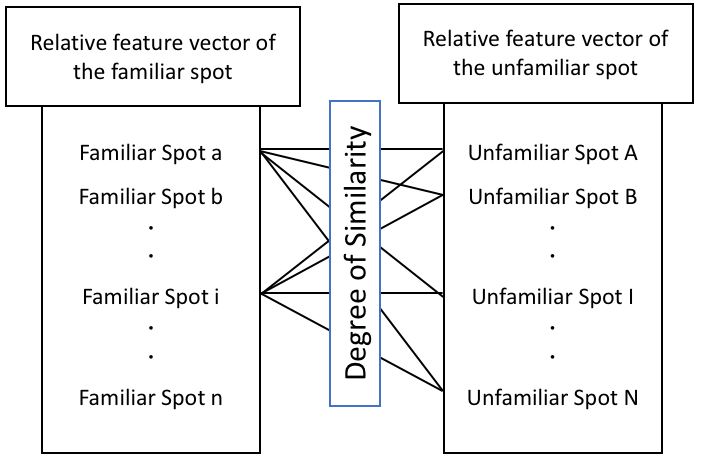
\includegraphics[clip,width=7.5cm,bb=0 0 720 540]{picture/Photo_CosSim_eng.png}
    % 類似度計算概念図
    \caption{Concept of similarity calculation}
    \label{fig:Photo_CosSim}
    \end{center}
\end{figure}

% 本研究では,観光スポットの特徴は相対的な特徴を利用する.
In this research, features of tourist spots make use of relative features.
% 相対的な特徴とは,特定の観光スポットが,ある観光スポット集合に含まれた他の観光スポットと比較した場合における独特な特徴である.
We define that the relative feature is a unique feature when a tourist spot is compared with other tourist spots in a set of tourist spots.
% 例として,観光スポット集合内に鹿苑寺と清水寺が存在する場合を考える.
As an example, we consider the case where there are ``Kinkakuji Temple'' and ``Kiyomizudera Temple'' in the set of tourist spots.
% このとき鹿苑寺の特徴は,金色,金箔,輝き等である.
At this time, the features of ``Kinkakuji Temple'' are gold color, gold leaf, glow, and so on.
% 一方,清水寺の特徴は,舞台,胎内,一望等である.
On the other hand, the features of ``Kiyomizudera Temple'' are the stage, the womb inside, the panoramic view, and so on.
% どちらも京都に存在する寺院であるため,京都や寺院に関連する特徴は独特な特徴として現れることがない.
Because both are temples existing in Kyoto, features related to Kyoto and temples do not appear as unique features.
% 次に,観光スポット集合内に東京都庁舎展望台と鹿苑寺が存在する場合を考える.
Next, we consider the case where ``the Tokyo Metropolitan Government Building Observatories'' and ``Kinkakuji Temple'' exist within the set of tourist spots.
% このとき,鹿苑寺の特徴は,金閣寺,お寺,金色,京都等である.
At this time, features of ``Kinkakuji Temple'' is Kinkakuji, a temple, golden color, Kyoto, and so on.
% 一方,東京都庁舎の特徴は,展望,夜景,新宿等である.
On the other hand, features of ``the Tokyo Metropolitan Government Building Observatories'' is perspectives, night view, Shinjuku, and so on.
% 観光スポットのカテゴリーが大きく異なる場合であれば,カテゴリーとしての特徴が現れる.
If the categories of tourist spots are largely different, features as categories will appear.
% また,スポット自体の特徴を表示することもできる。
Also, it can show the features of the spot itself.
% 本研究では,あるスポットが集合内の他のスポットと比較するとき,より各スポットの特徴を明らかにできる相対的な特徴に着目して研究を行う.
In this research, when a certain spot compares with other spots in the set, we focus on the relative features that make it possible to clarify the features of each spot.

% スポット差分ベクトルは式\ref{math:Vector difference}として定義される.
The relative feature vector $r_{state,i}$ is defined as formula \ref{math:Vector difference}.
% スポット差分ベクトルを求めるスポットを除いたスポット集合の各スポットのスポットベクトルの平均値を引いた値となる.
Is the value obtained by subtracting the average value of the spot vectors of the spots of the set of spots excluding the spot for which the relative feature vector is found.
% $S_{state} =\{s_1,s_2,\dots,s_n\}$は既訪問スポット集合や未訪問スポット集合となっている.
$S_{state} =\{s_1,s_2,\dots,s_n\}$ is a familiar spot set or an unfamiliar spot set.
% $state$は$'f'$のとき,既訪問スポット集合と定義する.
When $state$ is $'f'$, it means familiar spot set.
% $state$は$'u'$のとき,未訪問スポット集合と定義する.
When $state$ is $'u'$, it means unfamiliar spot set.
% $s_i$は集合$S_{state}$の観光スポットの特徴ベクトルを示している.
$s_i$ is a feature vector of a tourist spot in the set $S_{state}$.

\begin{equation}
  r_{state,i}=s_i-average(S_{state}-s_i)
  \label{math:Vector difference}
\end{equation}


%%%%%%%%%%%%%%%%%%%%%%%%%%%%%%%%%%%%%%%%%%
%説明スポットの決定
\subsection{Determination of explainable spot}
\label{subsec:Determination of explainable spot}

% 既訪問スポットの各特徴差分ベクトル$v_i$と未訪問スポットの各特徴差分ベクトル$v_j$から,既訪問スポットと未訪問スポット間の相対的な特徴の類似度(図\ref{fig:photo_cossim})を求める.
From the relative feature vector $r_{f,i}$ of the familiar spot and the relative feature vector $r_{u,j}$ of the unfamiliar spot, the relative feature similarity between the familiar spot and the unfamiliar spot (Fig. \ref{fig:Photo_CosSim} ).
% 類似度計算には,コサイン尺度(式\ref{math:CosSim})を用いる.
For the similarity calculation, use the cosine scale (formula \ref{math:CosSim}).

\begin{eqnarray}
  cos(r_{f,i},r_{u,j})=\frac{r_{f,i} \cdot r_{u,j}}{|r_{f,i}| \times |r_{u,j}|}
  \label{math:CosSim}
\end{eqnarray}

% 既訪問スポットの各特徴ベクトルと未訪問エリア内の各特徴ベクトルの類似度が0.125以上かつ,類似度が最も高い既訪問スポットと未訪問スポットの関連付けを行う.
A correlation between the familiar spot having similarity of each feature vector of the familiar spot and each feature vector in the unfamiliar area of 0.125 or more and the highest similarity and the unfamiliar spot is performed.
% また,既訪問スポットと未訪問スポットとの関連をつけるとき以下の2つの方法がある.
In addition, there are two ways to establish an association between a familiar spot and an unfamiliar spot.

\begin{enumerate}
  % \item 既訪問スポットをベースにして未訪問スポットと関連付ける方法
  \item how to relate to unfamiliar spots based on familiar spots
  % \item 未訪問スポットをベースにして既訪問スポットと関連付ける方法
  \item how to relate to familiar spots based on unfamiliar spots
\end{enumerate}

% 方法1では,既訪問スポットをベースにすると未訪問エリア内のスポットが複数の特徴を保持する場合は同じ未訪問スポットと関連付ける場合がある.
In the method 1, if the spot in the unfamiliar area holds a plurality of features when using the familiar spot as the base, there are cases where the spot is associated with the same unfamiliar spot.
% 方法2では,未訪問スポットをベースにすることによって,既訪問スポット集合から各スポットの特徴を取り出し,未訪問スポットと関連付けることができるため,方法2を利用する.
In method 2, method 2 is used as it is possible to extract features of each spot from the familiar spot set based on the unfamiliar spot and associate with the unfamiliar spot.
% また,本研究では,未訪問スポットを説明するため未訪問スポットをベースにすることが妥当と考えられる.
In addition, in this research, we considered that it is reasonable to base on unfamiliar spots for explaining unfamiliar spots.

%%%%%%%%%%%%%%%%%%%%%%%%%%%%%%%%%%%%%%%%%%
% 説明するための役割語の抽出
\subsection{Extraction of explainable words for role}
\label{subsec:Extraction of explainable words for role}
% 観光スポットのレビューはすべて形態素解析器「mecab-ipadic-NEologd」を使用することで,単語抽出処理を行う.
All tourist spots review words by using morphological analyzer ``mecab-ipadic-NEologd''.
% しかし,これらを用いて得られた単語は,日本語として成立しない語が含まれており,これらノイズの削除が必要となる.
However, words obtained by using these words contain words that do not hold Japanese, and it is necessary to delete these noises.
% 具体的には,助詞,助動詞,連体詞,記号,ストップワードを削除する.
Specifically, delete particles, auxiliary verbs, rentaishi, symbols, stopwords.

% 節\ref{subsec:Determination of explainable spot}で関連付けした既訪問スポットと未訪問スポットの情報はキーワード集合としてユーザに提示する.
We show the explanation information of the familiar spot and the unfamiliar spot associated in section \ref{subsec:Determination of explainable spot} to the user as the set of keywords.
% スポット内のキーワード特徴値は,式\ref{math:TFIDF}で定義する.
We calculate the feature value of a keyword in a spot is defined by the formula \ref{math:TFIDF}.
\begin{equation}
  TFIDF(t,d,state) = TF(t,d) \times log\Biggr(\frac{|S_{state}|}{DF(t,state)}\Biggr)
  \label{math:TFIDF}
\end{equation}
% $TF(t,d)$は,文書$d$内の単語$t$の値を返している.
Where function $TF(t,d)$ returns the number of the keyword $t$ in the document $d$.
% $d$は,スポットのすべ手のレビューを1つにまとめた文書である.
$d$ is a document combining all reviews of a spot into one.
% $DF(t,state)$は,キーワード$t$を含む文書の数である.
Function $DF(t,state)$ retuns the number of documents that include keyword $t$.
$|S_{state}|$ is the total number of spots.

% 本手法では,既訪問スポットに関して,ユーザが複数個のスポットを入力する.
In this method, for familiar spots, the user inputs plurality of spots.
% それぞれのスポットの全レビューをまとめて1つの文書と見なし,それ以外のスポットの全レビューも文書とみなすことで,式\ref{math:TFIDF}によってTFIDF値を算出し,既訪問スポット毎の特徴語とする.
By considering all reviews of each spot as one document at a time and by considering all reviews of the other spots as documents, the TFIDF value is calculated by the formula \ref{math:TFIDF}, and use it as the feature words for each spot in the unfamiliar area.

% 未訪問エリアに関して,ユーザがエリアを指定して入力する.
Regarding the unfamiliar area, the user designates an area and inputs it.
% エリア内のそれぞれのスポットの全レビューをまとめて1つの文書と見なし,それ以外のスポットの全レビューも文書とみなすことで,式\ref{math:TFIDF}によってTFIDF値を算出し,未訪問エリアのスポット毎の特徴語とする.
By considering all reviews of each spot in the area as one document and considering all reviews of the other spots as a document, the TFIDF value is calculated by the formula \ref{math:TFIDF}, and use it as the feature words for each spot in the unfamiliar area.

% 関連付けした既訪問スポットと未訪問スポットの説明情報は,TFIDFで求めた各スポットの特徴語による調和平均を用いて決定する.
The explanation information on the associated familiar spots and unfamiliar spots associated with each other is determined by using harmonic averages according to feature words of each spot obtained by TFIDF.
% 調和平均とは,逆数の算術平均の逆数である.
The harmonic mean is the reciprocal of the arithmetic mean of the reciprocal.
% 既訪問スポットのレビュー文書と,未訪問スポットのレビュー文書に,共通して出現する単語を抽出する.
We extract commonly appearing words in the review document of the familiar spot and the unfamiliar spot.
% 抽出した単語のスコアは式\ref{math:Harmonic Mean}によって定義する.
The score of the extracted word is defined by the formula \ref{math:Harmonic Mean}.
% $word_{familiar}$と$word_{unfamiliar}$は同じ単語がそれぞれ既訪問スポットのTFIDF値と未訪問スポットのTFIDF値を示している.
$TFIDF(t,d,f)$ and $TFIDF(t,d,u)$ indicate the TFIDF value of the familiar spot and the TFIDF value of the unfamiliar spot, respectively.
% 単語スコアの値が大きと既訪問スポットと未訪問スポットのそれぞれのTFIDF値が大きい,つまり単語がそれぞれの文書に置いて重要度が高いことを示している.
When the value of the word score is large, the TFIDF value of each of the familiar spot and the unfamiliar spot is large, that is, the word has high importance in each document.
% よって,単語スコアの上位10個の単語を説明情報としてユーザに提示する(図\ref{fig:photo_map}).
Therefore, the top ten words of the word score are presented to the user as explanation information (Fig. \ref{fig:photo_map}).

\begin{eqnarray}
  score(t,d) = \frac{2 \times TFIDF(t,d,f) \times TFIDF(t,d,u)}{TFIDF(t,d,f) + TFIDF(t,d,u)}
  \label{math:Harmonic Mean}
\end{eqnarray}

\begin{figure}[t]
  \begin{center}
    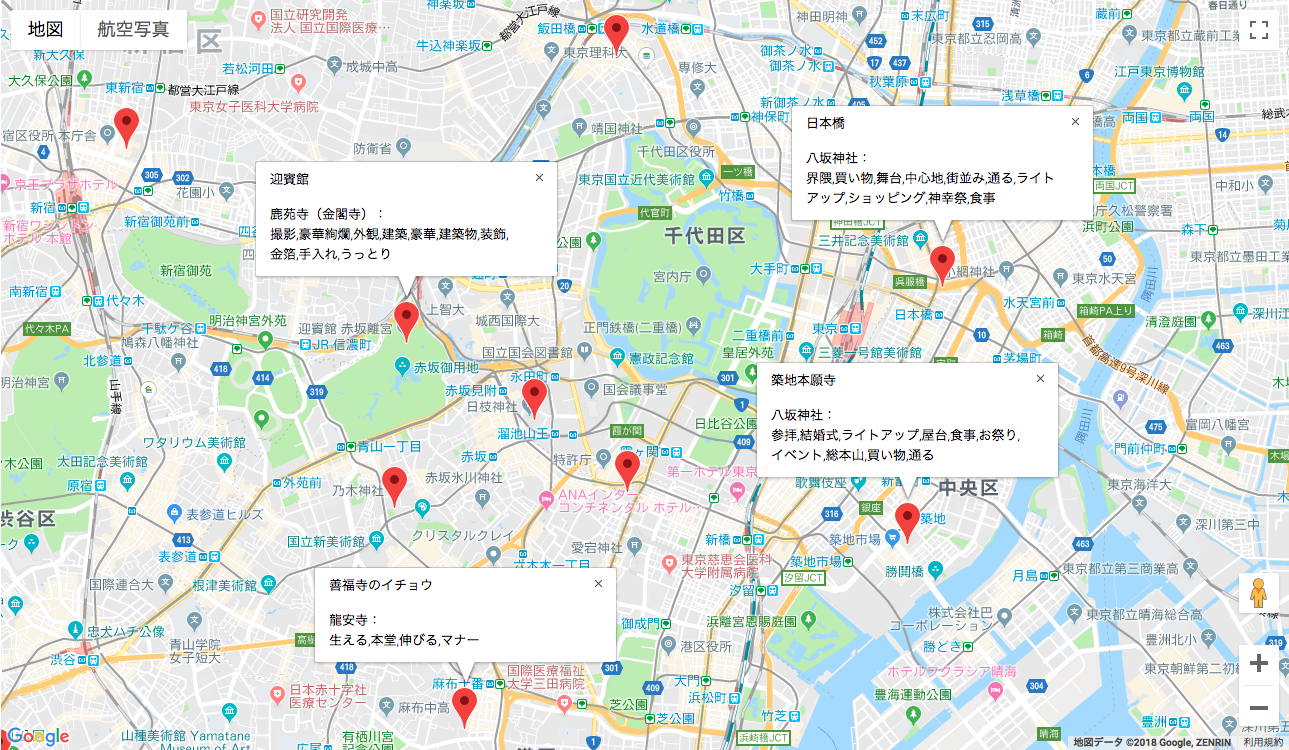
\includegraphics[clip,width=8.5cm,bb=0 0 1289 750]{picture/Photo_Map.png}
    \caption{Output interface}
    \label{fig:photo_map}
   \end{center}
\end{figure}


%%%%%%%%%%%%%%%%%%%%%%%%%%%%%%%%%%%%%%%%%%
\subsection{Example of explained unfamiliar spots}
\label{subsec:Example of explained unfamiliar spots}

\begin{table}[t]
  \caption{Familiar spot group and Unfamiliar spot group}
  \label{table:Familiar spot group and Unfamiliar spot group}
  \centering
  \begin{tabular}{l|l}
  \hline
  \multicolumn{1}{c|}{Familiar Spot Name} & \multicolumn{1}{c}{Unfamiliar Spot Name} \\ \hline
  Sensoji Temple                          & Tokyo Disneyland (R)                     \\
  Odawara-jo Park                         & Shinjuku Gyoen                           \\
  Fushimiinari-taisha Shrine              & Tokyo Skytree                            \\
  Nara Park                               & Tokyo Tower Main Deck            \\
  Mishima Skywalk                         & Meiji Jingu                              \\ \hline
  \end{tabular}
\end{table}

\begin{table*}[t]
  \caption{Explanation information}
  \label{table:Explanation information}
  \centering
  \begin{tabular}{l|l|l}
  \hline
  \multicolumn{1}{c|}{Unfamiliar Spot} & \multicolumn{1}{c|}{Familiar Spot} & \multicolumn{1}{c}{Explanation Information}                     \\ \hline
  % 新宿御苑                      &  小田原城址公園                        & お花見,咲き誇る,園内,桜の時,のんびり,手入れ,自然,遊具,ツツジ          \\ \hline
  Shinjuku Gyoen                      & Odawara-jo Park                         & flower viewing, bloom, inside the park, cherry-blossoms, carefree, care, nature, play equipment, azalea          \\
  % 東京スカイツリー                     & 三島スカイウォーク                    & 富士山,揺れ,高所恐怖症,揺れる,天井,絶景,エレベーター,パノラマ,展望デッキ,昇る \\
  Tokyo Skytree                     & Mishima Skywalk                    & mount fuji, tremor, high fear, trembling, ceiling, magnificent view, elevator, panorama, observation deck, rising
 \\ \hline
  \end{tabular}
\end{table*}

% 表\ref{table:Familiar spots and Unfamiliar spots}は,ユーザが既に訪問したことがあるスポットと,未訪問スポットの集合の例である.
Table \ref{table:Familiar spot group and Unfamiliar spot group} is an example of a spot that a user has familiar spots and unfamiliar spots.

% 未訪問スポットは東京都内からランダムに選んだ5つのスポットである.
Unfamiliar spots are five spots randomly selected from within Tokyo.
% 節\ref{sec:An Explanation Method of Unfamiliar Tourist Spots}の提案手法を使って説明単語を求めた結果は表\ref{table:Explanation information}である.
Table \ref{table:Explanation information} shows the results of explaining the explanatory words using the proposed method in Section \ref{sec:An Explanation Method of Unfamiliar Tourist Spots}.

% 公園という特徴に注目すると,未訪問スポット集合内で最も公園に近いスポットは新宿御苑であると考えられる.
Focusing on the feature of the park, it is thought that the spot closest to the park in the unfamiliar spot group is ``Shinjuku Gyoen''.
% 既訪問スポット集合内には小田原城址公園と奈良公園の2つの公園がある.
In the set of familiar spots there are two parks, ``Odawara-jo Park'' and ``Nara Park''.
% 小田原城址公園には花や遊具に対する記述が多く,奈良公園は鹿や草に対する記述が多い.
``Odawara-jo Park'' has a lot of descriptions about flowers and play equipments, and there are many descriptions for deers and grass at ``Nara Park''.
% 新宿御苑は花や遊具に対する記述が多いため,小田原城址公園との関連性があると考えられる.
Because ``Shinjuku Gyoen'' has a lot of descriptions about flowers and play equipments, it seems to be related to ``Odawara-jo Park''.

% 三島スカイウォークは既訪問スポット集合内で眺めがいい,高いの特徴が一番強いことが考えられる.
``Mishima Skywalk'' has a view in the set of familiar spots, and it can be considered that the feature of the highest is the strongest.
% 未訪問スポット集合内で眺めがいい,高いの特徴が強いのは東京スカイツリーや東京タワー大展望台の2つがある.
There are two of ``Tokyo Skytree'' and ``Tokyo Tower Main Deck'' that have good views with a high view in the unfamiliar spot group.
% 東京スカイツリーはより高いによって三島スカイウォークと考えられるが,説明情報を見ると富士山が入っている.
``Tokyo Skytree'' is thought to be ``Mishima Skywalk'' to its higher level, but ``Mount Fuji'' is included when I look at the explanation information.
% 2つスポットの高さは富士山という単語によって強調されている.
The height of the two spots is highlighted by the word ``Mount Fuji''.
% 提案手法は各集合のスポット毎の特徴を表すことができる.
The proposed method can show the feature of each set of spots.



%%%%%%%%%%%%%%%%%%%%%%%%%%%%%%%%%%%%%%%%%%
%%%%%%%%%%%%%%%%%%%%%%%%%%%%%%%%%%%%%%%%%%
\section{Evaluation Experiment}
\label{sec:Evaluation Experiment}
%%%%%%%%%%%%%%%%%%%%%%%%%%%%%%%%%%%%%%%%%%
%%%%%%%%%%%%%%%%%%%%%%%%%%%%%%%%%%%%%%%%%%
\subsection{Settings of experiment}
\label{subsec:Settings of experiment}

% 絶対的な特徴と提案手法の相対的な特徴による説明情報を提示する方法の比較を行う.
We compare absolute features and methods to present explanatory information by relative features of the proposed method.
% また,相対的な特徴を利用する場合において,調和平均を利用して単語スコアを算出する方法と相加平均を利用して単語スコアを算出する方法の比較を行った.
In addition, in the case of using relative features, we compare the method of calculating word scores using harmonic mean and the method of calculating word score using arithmetic mean.

% クラウドソーシングのサービスである,CrowdWorks\footnote{https://crowdworks.jp/}を利用して24人の被験者を集めた.
We collected 24 subjects using CrowdWorks\footnote{https://crowdworks.jp/}, a crowdsourcing service.
% じゃらんで取得した観光スポットを使って,被験者の既訪問スポットの選択による未訪問スポットの説明情報の提示を行った.
We presented presentation information on unfamiliar spots by selecting subjects' familiar spots using tourist spots acquired by Jalan taking place.
% 絶対的な特徴と相対的な特徴の説明情報のパターンは以下の4つとなる.
The patterns of explanatory information of absolute feature and relative features are as follows.
\begin{description}
\item[A]Absolute feature (category, duration time, season)
\item[B]Absolute feature (feature vector)
\item[C]Relative features (relative feature vector, harmonic mean)
\item[D]Relative features (relative feature vector, arithmetic mean)
\end{description}

% 説明情報Aは,観光スポット検索サイトでスポットを検索するためで使う絞り込み情報である.絞り込み情報は例は以下の3つである.
The explanation information A is narrowing-down information used for searching spots on the sightseeing spots search site. Three examples of narrowing down information are as follows.

\begin{itemize}
\item category: Shrine / Temple,Tourist facilities / Tourist tours etc.
\item duration time: less than 1 hour,1\verb|~|2 hour etc.
\item season: 1\verb|~|12 month, spring, summer, autumn, winnter
\end{itemize}

% まず,既訪問スポットを使って,未訪問スポットとのカテゴリが一致がどうか,滞在時間と一致かどうか,訪問時期と一致かどうかの順で徐々に情報を絞って,既訪問スポットと未訪問スポットの対応付けを行う.
First, using the familiar spot, we gradually narrow down the information in order of whether the categories with unfamiliar spot match, whether it matches the duration time or not, and whether or not it matches the season, and the familiar and the unfamiliar spot.
% 次に,絞った後の未訪問スポットが複数残った場合,レビュー数が1番多い未訪問スポットを利用する.
Next, if there are multiple unfamiliar spots after squeezing, use the unfamiliar spot with the most review number.
% 最後に,節\ref{subsec:説明するための役割語の抽出}を使って説明するための役割語を抽出し,被験者に提示する.
Finally, we extract the role words for explanation using section \ref{subsec:Extraction of explainable words for role} and present them to the subjects.
% 説明情報Bは,節\ref{subsec:スポットのレビューから特徴ベクトル生成}で作成した特徴ベクトルを使って,各スポットの特徴とする.
The explanation information B is the feature of each spot using the feature vector created in section \ref{subsec:Generating feature vector using user reviews of spot}.
% 説明情報Cは,提案手法である.
The explanation information C is the proposed method.
% 説明情報Dは,関連付けした既訪問スポットと未訪問スポットの説明情報は,TFIDFで求めた各スポットの特徴語による調和平均を用いて決定する.
The explanation information D, explanation information on the familiar spot and the unfamiliar spot associated with each other is determined by using harmonic averages according to feature words of each spot obtained by TFIDF.
% 既訪問スポットのレビュー文書と,未訪問スポットのレビュー文書に,共通して出現する単語を抽出する.
We extracts commonly appearing words in the review document of the familiar spot and the unfamiliar spot.
% また,抽出した単語のはぞれぞれのスポットのTFIDFの値の平均を以上である必要がある.
In addition, it is necessary for the extracted word to have an average value of the TFIDF values ​​of the respective spots.
% 既訪問スポット単語のTFIDF値と未訪問スポット単語のTFIDF値の差の絶対値を単語スコアとして算出し,単語スコアが最も0に近い10個の単語を説明情報として被験者に提示する.
The absolute value of the difference between the TFIDF value of the familiar spot word and the TFIDF value of the unfamiliar spot word is calculated as the word score and ten words whose word score is the closest to 0 are posted on the subject as explanation information.

% まず,被験者は既に訪問したことがあり,気に入った観光スポットを4つ以上10つ以下入力した.
First, the subjects have familiar spot, favorite spot and enter between 4 to 10.
% 入力するスポットは,検索候補から選んでもらう.
The subjects have selected from the search candidates as the input spots.
% 例えば,新宿御苑---新宿,清水寺---京都などがある.
For example,Shinjuku Gyoen---Shinjuku, Kiyomizudera---Kyoto etc.
% 次に,被験者は旅行等で行ったことがなく,これから行ってみたい都道府県・エリアを入力した.
Next, the subjects never went on a trip etc and entered prefectures / areas that we would like to visit.
% 説明情報のパターンのAからDの順で処理を行って,ユーザに未訪問スポット名,キーワード,既訪問スポット名を提示し,以下の5つの評価から1つを選択した.
Processing was carried out in the order of A to D of the pattern of explanation information, and the unfamiliar spot name, keyword, and familiar spot name were presented to the user, and one of the following 5 evaluations was selected.
\begin{enumerate}
  \item No keyword.
  \item There is a relationship between the two spots in the first place, the relationship became clear by the keyword.
  \item To the relationship of the two spots noticed for the first time by keyword.
  \item There is a relationship between the two spots, but the keyword does not represent the relation.
  \item There is no relationship between the two spots.
\end{enumerate}

%%%%%%%%%%%%%%%%%%%%%%%%%%%%%%%%%%%%%%%%%%
\subsection{Result}
\label{subsec:Result}

\begin{table*}[t]
  \caption{Statistics on the number of data of experiment results}
  \label{table:Statistics on the number of data of experiment results}
  \centering
  \begin{tabular}{c|r|r|r|r|r}
  \hline
  Evaluation & \multicolumn{1}{c|}{Explanation information A} & \multicolumn{1}{c|}{Explanation information B} & \multicolumn{1}{c|}{Explanation information C} & \multicolumn{1}{c|}{Explanation information D} & \multicolumn{1}{c}{Total} \\ \hline
  1  & 0                      & 0                      & 0                      & 4                      & 4                      \\
  2  & 19                     & 44                     & 32                     & 26                     & 121                    \\
  3  & 20                     & 62                     & 53                     & 56                     & 191                    \\
  4  & 1                      & 3                      & 3                      & 3                      & 10                     \\
  5  & 6                      & 21                     & 21                     & 20                     & 68                     \\ \hline
  Total & 46                     & 130                    & 109                    & 109                    & 394                    \\ \hline
  \end{tabular}
\end{table*}

% 表\ref{table:Statistics on the number of data of experiment results}は評価1から5の説明情報AからDのそれぞれの実験結果のデータの数である.
Table \ref{table:Statistics on the number of data of experiment results} shows the number of data of each experimental result of explanation information A to D of Evaluations 1 to 5.
% 評価実験では,使用可能のデータの合計は394件である.
In the evaluation experiment, the total of usable data is 394.
% 説明情報Aの方が未訪問スポットと関連がある既訪問スポットの数が最も少ない.
The explanation information A has the smallest number of familiar spots associated with unfamiliar spots.
% 説明情報Bの方が未訪問スポットと関連がある既訪問スポットの数が最も多い.
The explanation information B has the largest number of familiar spots related to unfamiliar spots.
% 説明情報Cと説明情報Dについて,未訪問スポットと既訪問スポットの関連付け手法は同じであるため,数が同じとなる.
The explanation information C and explanation information D, the association method between the unfamiliar spot and the familiar spot is the same, so the numbers are the same.

\begin{table*}[t]
  \caption{Percentage of evaluation in explanation information}
  \label{table:Percentage of evaluation in explanation information}
  \centering
  \begin{tabular}{c|r|r|r|r}
  \hline
  Evaluation & \multicolumn{1}{c|}{Explanation information A} & \multicolumn{1}{c|}{Explanation information B} & \multicolumn{1}{c|}{Explanation information C} & \multicolumn{1}{c}{Explanation information D} \\ \hline
  1  & 0.00\%                     & 0.00\%                     & 0.00\%                     & 3.67\%                    \\
  2  & 41.30\%                    & 33.85\%                    & 29.36\%                    & 23.85\%                   \\
  3  & 43.48\%                    & 47.69\%                    & 48.62\%                    & 51.38\%                   \\
  4  & 2.17\%                     & 2.31\%                     & 2.75\%                     & 2.75\%                    \\
  5  & 13.04\%                    & 16.15\%                    & 19.27\%                    & 18.35\%                   \\ \hline
  \end{tabular}
\end{table*}

% 表\ref{table:Percentage of evaluation in explanation information}は説明情報AからDにおいて評価1から5の実験結果のデータの数の割合である.
Table \ref{table:Percentage of evaluation in explanation information} shows the ratio of the number of data of the experiment results as the evaluation 1 to 5 in the explanation information A to D.
% 被験者に提示する説明情報Aは,未訪問スポットと既訪問スポットがそもそも関連性があり,またキーワードを提示することによってさらに明確となった.
The explanatory information A presented to subjects, the unfamiliar spot and the familiar spot were originally related, and further clarified by presenting keywords.
% 説明情報Dは,未訪問スポットと既訪問スポットに関連性がないと思っていたが,被験者にキーワードを提示することによって初めて気がついたため,本研究の提案手法に関連性がある.
The explanatory information D thought that there was no relevance to the unfamiliar spot and the familiar spot, but since it was noticed for the first time by presenting the keyword to the subject, it is related to the proposed method of this research.
% 説明情報Cと説明情報Dは,被験者に提示する未訪問スポットと既訪問スポットがそもそも関連性がない割合が多い.
In explanation information C and explanation information D, there are many proportions in which the unfamiliar spot presented to the subject and the familiar spot are not related in the first place.
% 4つの説明情報パターンにおいて説明情報Dのみ被験者に提示するキーワードがない.
In the four explanatory information patterns, only the explanatory information D has no keyword to present to the subject.
% よって,調和平均を利用することによって 被験者にキーワードを提示することができる場合が多いといえる.
Therefore, it can be said that in many cases it is possible to present keywords to subjects by using harmonic means.
% また,評価1,評価4と評価5は説明情報を意味がなしていないことが示すことができる.
In addition, it can be shown that evaluation 1, evaluation 4 and evaluation 5 mean that explanation information is meaningless.
% よって,説明情報Dは最もの意味をなしていないことがいえる.
Therefore, it can be said that explanation information D does not make the most sense.

% 評価1と評価2はから,被験者に提示する未訪問スポットと既訪問スポットがそもそも関連性があるカテゴリを利用する場合が1番良いでる.
From evaluation 1 and evaluation 2, the best case is to use categories that are unfamiliar spots presented to subjects and familiar spots in the first place.
% しかし,関連性のあるスポットの数はカテゴリに制限しているため被験者に提示できる数も少ない.
However, since the number of relevant spots is limited to categories, there are also few numbers that can be presented to subjects.
% また,別カテゴリのスポット情報を被験者に提示できないため意外性を求めることができないといえる.
In addition, it can not be said that unexpectedness can not be obtained because spot information of another category can not be presented to subjects.
% 2番目は特徴ベクトル利用する場合,3番目は差分ベクトルと調和平均の組み合わせるとき,最も良くないのは説明情報Dの差分ベクトルと相加平均の組み合わせである.
The second is to use the feature vector, the third to combine the relative feature vector and the harmonic mean, the combination which is not the best is the combination of the relative feature vector of the explanation information D and the arithmetic mean.
% 説明情報Cと説明情報Dの関連性があるスポットの数が同じであるが,相加平均を使って単語スコアを算出することによって被験者に提示するキーワードの理解支援の役割が減少したといえる.
Although the number of spots with relevance between explanation information C and explanation information D is the same, it can be said that the role of understanding support of keywords presented to subjects is reduced by calculating word scores using arithmetic mean.

% 評価2は差分ベクトルと相加平均の組み合わせが最も良い,差分ベクトルと調和平均の組み合わせが2番目良い,3番目は特徴ベクトル利用する場合,最も良くないのはカテゴリを用いる場合である.
Evaluation 2 is the combination of the relative feature vector and arithmetic mean, the combination of the relative feature vector and the harmonic mean is the second best, the third is the case where the feature vector is used, and the case where the category is not the best is used.
% よって,説明情報Bの特徴ベクトルと説明情報Cの差分ベクトルと調和平均の組み合わせが良い結果を示すことができるといえる.
Therefore, it can be said that a combination of a relative feature vector between the feature vector of the explanation information B and the explanation information C and a harmonic mean can show a good result.
% また,差分ベクトルを利用することによって被験者に意外性があり,カテゴリに拘らない未訪問スポットを提示することができる.
In addition, by using the relative feature vector, subjects have unexpectedness, and it is possible to present unfamiliar spots irrespective of categories.

\begin{table*}[t]
  \caption{When the categories of the familiar spots are different or  percentage of evaluation when similar}
  \label{table:When the categories different or similar}
  \centering
  \begin{tabular}{c|r|r}
  \hline
  & \multicolumn{1}{c|}{\begin{tabular}[c]{@{}c@{}}When the familiar spots are different\end{tabular}} & \multicolumn{1}{c}{\begin{tabular}[c]{@{}c@{}}When the familiar spots are similar\end{tabular}} \\ \hline
  Explanation information B \& Evaluation 1 & 56.82\%                            & 43.18\%                            \\
  Explanation information C \& Evaluation 1 & 71.87\%                            & 28.13\%                            \\ \hline
  Explanation information B \& Evaluation 2 & 51.61\%                            & 48.39\%                            \\
  Explanation information C \& Evaluation 2 & 52.83\%                            & 47.170\%                            \\ \hline
\end{tabular}
\end{table*}

% 説明情報Bと説明情報Cについて,被験者が入力した既訪問スポットのカテゴリが異なる場合と類似する場合のとき,評価2と評価3の評価の割合は表\ref{table:When the categories of the familiar spots are different and percentage of evaluation when similar}となる.
For explanation information B and explanation information C, the case where the category of the familiar spot inputted by the examinee is different is similar to the case where the categories of the familiar spots input by the subject are different, the ratio of the evaluation of the evaluation 2 and the evaluation 3 is the table \ref{table:When the categories different or similar}.
% 提案手法である説明情報Cを使うと,被験者が既に訪問したあるスポットと関係なしで,被験者が有意味のキーワードを提示することができる.
Using explanation information C, which is the proposed method, subjects can present meaningful keywords without relation to a certain spot that the subject has familiar visited.
% 差分ベクトルを利用することによって,カテゴリに渡って各スポットの特徴を求めることができるといえる.
By using the relative feature vector, it can be said that the characteristics of each spot can be found over the category.
% 既訪問スポットのジャンルが類似する場合では説明情報Bの方かより良い評価となっている.
In the case where the genres of the familiar visited spots are similar, the explanation information B is better than the case.


%%%%%%%%%%%%%%%%%%%%%%%%%%%%%%%%%%%%%%%%%%
%%%%%%%%%%%%%%%%%%%%%%%%%%%%%%%%%%%%%%%%%%
\section{Conclusions and Future Work}
\label{sec:Conclusions and Future Work}
%%%%%%%%%%%%%%%%%%%%%%%%%%%%%%%%%%%%%%%%%%
%%%%%%%%%%%%%%%%%%%%%%%%%%%%%%%%%%%%%%%%%%
% 本研究では,ユーザが行きたい観光スポットが決まっていない場合,ランキング,おすすめ情報やカテゴリなどに観光検索情報を使用することによって,検索した観光スポットがに対する理解が困難であることを着目した.
We focused on the difficulty of understanding the tourist spots searched by using the tourist spot search engine in ranking, recommendation information, categories, and so on., if the presented tourist spots are unfamiliar for the user.
% 未訪問スポットに対する理解を支援するために,ユーザが既に訪問したことがあるスポットの特徴を未訪問スポットにあてはめて理解を支援する説明手法を提案した.
In order to support understanding of unfamiliar spots, we proposed an explanatory method to support understanding by comparing unfamiliar spots with familiar spots that users have already visited.

% 評価実験では4つの説明情報パターンを用いて比較を行った.
In the evaluation experiment, we evaluate four method of explanatory information.
% 結果,カテゴリを利用する場合では,未訪問スポットと関連する既訪問スポットが最も少ない.
As a result, in the case of using categories, the number of familiar spots associated with unfamiliar spots is the smallest.
% 差分ベクトルと相加平均を利用する場合では,キーワードの理解を支援する役割が最も少ない.
In the case of using the relative feature vector and arithmetic mean, the role of supporting the understanding of keywords is the least.
% 差分ベクトルと調和平均を利用することによって,各スポットの特徴を求めることができる.
By using the relative feature vector and harmonic mean, the characteristics of each spot can be obtained.
% また,意外性がある未訪問スポットと既訪問スポットを関連付けることができ,ユーザが知らない観光スポットに対する興味と関心を引き出すことができる可能性があることを確認した.
In addition, we confirmed that it was possible to correlate unexpected unfamiliar spots with familiar spots, and that there is a possibility that interest and attention can be drawn to tourist spots that users do not know.

% 今後の課題としては,実験時に得られたユーザに提示するキーワード,未訪問スポットと既訪問スポットのカテゴリの関連性を分析する.
As future works, we analyze experimental result such as the relevance between keywords presented to users.
% また,ユーザに提示する各キーワードの有効性と関連性についての評価を行う予定である.
We also plan to evaluate the effectiveness and relevance of each keyword presented to the user.


% use section* for acknowledgement
\section*{Acknowledgment}
This work was supported by ISPS KAKENHI of Grant-in-Aid for Scientific Research(C) Grant Number 18K11551.


% Can use something like this to put references on a page
% by themselves when using endfloat and the captionsoff option.
\ifCLASSOPTIONcaptionsoff
  \newpage
\fi



% trigger a \newpage just before the given reference
% number - used to balance the columns on the last page
% adjust value as needed - may need to be readjusted if
% the document is modified later
%\IAENGtriggeratref{8}
% The "triggered" command can be changed if desired:
%\IAENGtriggercmd{\enlargethispage{-5in}}

% references section

% can use a bibliography generated by BibTeX as a .bbl file
% BibTeX documentation can be easily obtained at:
% http://www.ctan.org/tex-archive/biblio/bibtex/contrib/doc/
% The IAENGtran BibTeX style support page is at:
% http://www.michaelshell.org/tex/IAENGtran/bibtex/
%\bibliographystyle{IAENGtran}
% argument is your BibTeX string definitions and bibliography database(s)
%\bibliography{IAENGabrv,../bib/paper}
%
% <OR> manually copy in the resultant .bbl file
% set second argument of \begin to the number of references
% (used to reserve space for the reference number labels box)
\begin{thebibliography}{1}
  \bibitem{Codd01}
    T. Kurashima, T. Iwata, G. Irie and K. Fujimura.,
      ``Travel route recommendation using geotags in photo sharing sites'',
      CIKM '10 Proceedings of the 19th ACM international conference on Information and knowledge management, pp.579-588, 2010
  \bibitem{Codd02}
    R. Kitamura and T. Itoh,
      ``Tourist Spot Recommmendation Applying Generic Object Recognition with Travel Photos'',
      ITE Tech. Rep., Vol.42, No.12, AIT2018-94, pp.185-188, 2018
  \bibitem{Codd03}
    A. J. Cheng, Y. Y. Chen, Y. T. Huang and Winston H. Hsu,
      ``Personalized Travel Recommendation by Mining People Attributes from Community-Contributed Photos'',
      MM '11 Proceedings of the 19th ACM international conference on Multimedia, pp.83-92, 2011
  \bibitem{Codd04}
    K. J. Holyoak and P. Thagard,
      ``Mental Leaps: Analogy in Creative Thought, MIT Press'',
      % Cambridge, 1995 %英語用
      Journal of Japanese Society for Artificial Intelligence,  Vol.11, No.3,  pp.489, 1996
  \bibitem{Codd05}
    D. Gentner,
      ``Structure-Mapping: A Theoretical Framework for Analogy'',
      Cognitive Science, Vol.7, pp.155–170, 1983
  \bibitem{Codd06}
    M. L. Gick and K. J. Holyoak,
      ``Analogical Problem Solving'',
      Cognitive Psychology, Vol.12, pp.306–355, 1980
  \bibitem{Codd07}
    M. L. Gick and K. J. Holyoak,
      ``Scheme Induction and Similarity in Analogical Transfer'',
      Cognitive Psychology, Vol.15, pp.1–38, 1983
  \bibitem{Codd08}
    Z. Chen and M. W. Daehler,
      ``Positive and Negative Transfer in Analogical Problem-solving by 6-years-old Children'',
      Cognitive Development, Vol.4, No.4, pp.327–344, 1989
  \bibitem{Codd09}
    K. J. Holyoak and P. Thagard,
      ``Analogical Mapping by Constraint Satisfaction'',
      Cognitive Science, Vol.13, pp.295–355, 1989
  \bibitem{Codd10}
    Quoc V. Le and Tomas Mikolov,
      ``Distributed representations of sentences and documents'',
      In Proceedings of the 31th International Conference on Machine Learning, ICML 2014, pp. 1188–1196, 2014
  \bibitem{Codd11}
    % 日本の形態素解析に条件付きランダムフィールドを適用する
    T. Kudo, K. Yamamoto and Y. Matsumoto,
    ``Applying Conditional Random Fields to Japanese Morphological Analysis'',
    Proceedings of the 2004 Conference on Empirical Methods in Natural Language Processing (EMNLP-2004), pp.230-237, 2004

\end{thebibliography}


\end{document}
